%! Author = trevo
%! Date = 2/22/2025

% Preamble
\documentclass[12pt]{report}
\usepackage{amsmath,geometry,setspace, enumerate,pdfpages,mathrsfs,hyperref,csquotes,graphicx,amsfonts,pdfpages}
\usepackage[british]{babel}
\usepackage[round]{natbib}
\bibliographystyle{plainnat}
\doublespacing
\setlength\parindent{24pt}
\setcounter{tocdepth}{3}



\begin{document}

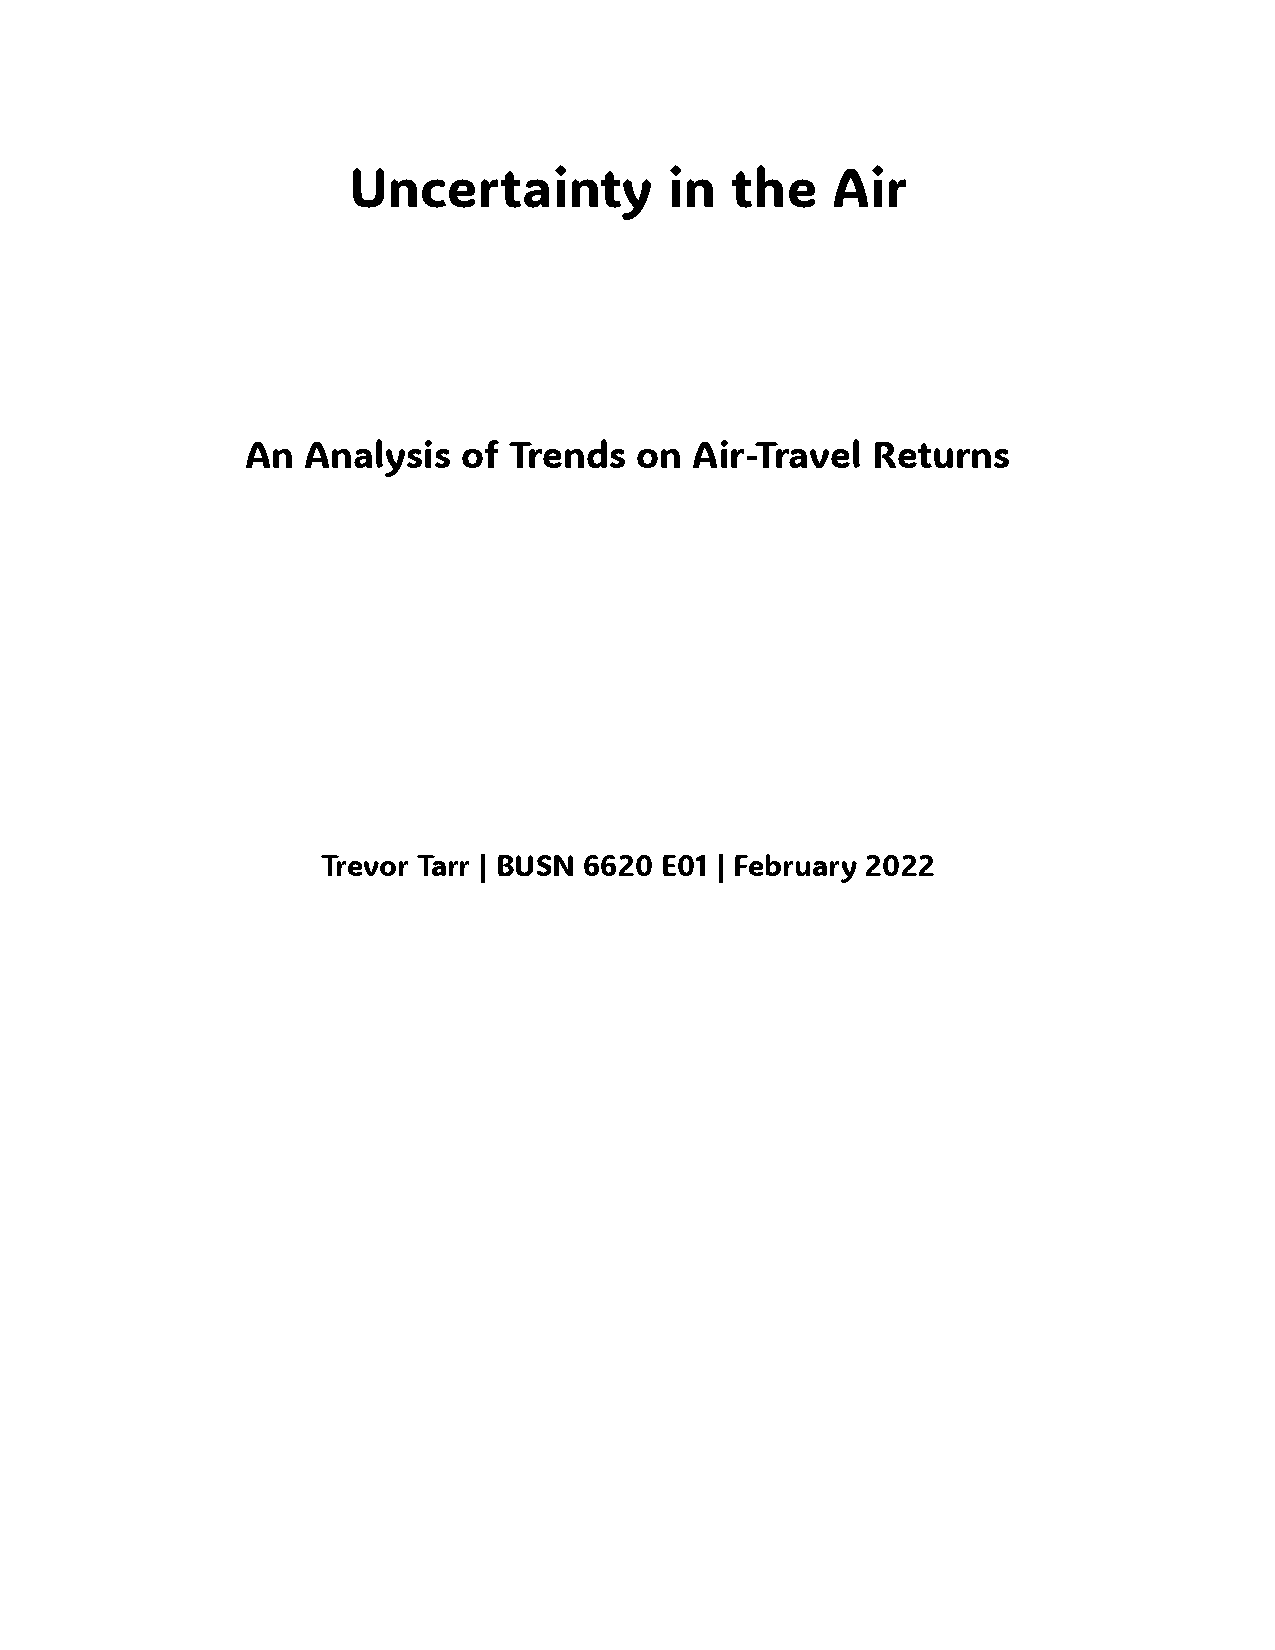
\includepdf{pdfFinalCoverPage}
    \newpage
\pagenumbering{gobble}
    \newpage
    \pagenumbering{roman}


\newpage
\tableofcontents
\newpage

\pagenumbering{arabic}
\chapter*{Abstract, Hypothesis, Motivation}
\addcontentsline{toc}{chapter}{Abstract, Hypothesis, Motivation}
\section*{\underline{Abstract}}
\addcontentsline{toc}{section}{Abstract}

\section*{\underline{Hypothesis}}
\addcontentsline{toc}{section}{Hypothesis}

\section*{\underline{Motivation}}
\addcontentsline{toc}{section}{Motivation}

\nocite{*}

\newpage
\chapter*{Methodology}
\section*{\underline{Variables}}
\begin{enumerate}
    \item[Dependent]: Airline Closing Monthly Stock Prices. The airlines chosen are a sample from both Legacy and Low-Cost carriers as to observe trend data on both sectors within the industry.
    \begin{enumerate}
        \item[Legacy]:
            \begin{enumerate}
                \item[1.]Delta Air Lines, Inc. (DAL)
                \item[2.]United Airlines Holdings, Inc. (UAL)
            \end{enumerate}
        \item[Low-Cost]:
            \begin{enumerate}
                \item[3.]Southwest Airlines Co. (LUV)
                \item[4.]Allegiant Travel Company (ALGT)
            \end{enumerate}
    \end{enumerate}
    \item[Independent]: Trend Data (Google Trend Data).
    These trend topics are to encapsulate various issues, risks, and interests theorized to impact the airline market.
        \begin{enumerate}
            \item[Travel Restriction]:
            \item[Boeing Plane]:
            \item[Airbus Plane]:
            \item[Pilot Strike]:
            \item[Terrorism]:
        \end{enumerate}
    \tiny Note: Singular was chosen over plural to account for seperated events involving planes, strikes, and restrictions.
\end{enumerate}
\section*{\underline{Data Collection}}

Data collection for Dependent Variables was gathered from Historical Data from Yahoo Finance using tickers: UAL, DAL, LUV, ALGT. This data was then transferred to a Microsoft Excel notebook.
\\ \\
Data collection for Independent variables were gathered from worldwide monthly Google Trend data values over the maximum amount stored by Google Trends (2004 onwards).
This data was downloaded as a .csv file and opened and used in a separate Microsoft Excel sheet in the same notebook as the Dependent variable data.

\newpage
\chapter*{Results and Interpertations}
\addcontentsline{toc}{chapter}{Results and Interpertations}

\section*{\underline{United}}
\addcontentsline{toc}{section}{United}
\subsection*{Results:}
\begin{enumerate}
    \item
    \item
    \item
    \item
\end{enumerate}
\subsection*{Interpretation:}

\newpage
\section*{\underline{Delta}}
\addcontentsline{toc}{section}{Delta}
\subsection*{Results:}
\begin{enumerate}
    \item
    \item
    \item
    \item
\end{enumerate}
\subsection*{Interpretation:}

\newpage
\section*{\underline{Southwest}}
\addcontentsline{toc}{section}{Southwest}
\subsection*{Results:}
\begin{enumerate}
    \item
    \item
    \item
    \item
\end{enumerate}
\subsection*{Interpretation:}

\newpage
\section*{\underline{Allegiant}}
\addcontentsline{toc}{section}{Allegiant}
\subsection*{Results:}
\subsection*{Interpretation:}

\newpage


\chapter*{Conclusion, Recommendations, \& Bibliography}
\addcontentsline{toc}{chapter}{Conclusion, Recommendations \& Bibliography}
\section*{Conclusion}
\addcontentsline{toc}{section}{Conclusion}

\section*{Recommendations}
\addcontentsline{toc}{section}{Recommendations}
\newpage




\addcontentsline{toc}{section}{Bibliography}

    \bibliography{resources}
\end{document}
